%! Author = ACA
%! Date = 11-Sep-21

% Preamble
\documentclass[a4paper]{report}
\usepackage[a4paper, head=43pt, margin=0.9in]{geometry}

% Generated constants
\input{snip/constants}

% Utilities
%! Author = ACA
%! Date = 11-Sep-21

% Packages
\usepackage{blindtext}
\usepackage{hyperref}
\usepackage{underscore} % So underscores don't have to escaped in text mode
\usepackage[toc,page]{appendix}
\usepackage[acronym,hyperfirst=false]{glossaries}
\usepackage{glossary-longbooktabs}
\usepackage{longtable}

%%%%%%%%%%%%%%%%%%
% Levels
\newcounter{currentlevel}
\newcounter{nextlevel}

\makeatletter
\newcommand\level[1]{%
  \setcounter{currentlevel}{#1}%
  \setcounter{nextlevel}{#1}%
  \addtocounter{nextlevel}{1}%
  \ifcase#1\relax\expandafter\chapter\or
    \expandafter\section\or
    \expandafter\subsection\or
    \expandafter\subsubsection\else
    \def\next{\@level{#1}}\expandafter\next
  \fi}
\newcommand{\@level}[1]{%
  \@startsection{level#1}
    {#1}
    {\z@}%
    {-3.25ex\@plus -1ex \@minus -.2ex}%
    {1.5ex \@plus .2ex}%
    {\normalfont\normalsize\bfseries}}

\newdimen\@leveldim
\newdimen\@dotsdim
{\normalfont\normalsize
 \sbox\z@{0}\global\@leveldim=\wd\z@
 \sbox\z@{.}\global\@dotsdim=\wd\z@
}

\newcounter{level4}[subsubsection]
\@namedef{thelevel4}{\thesubsubsection.\arabic{level4}}
\@namedef{level4mark}#1{}
\def\l@section{\@dottedtocline{1}{0pt}{\dimexpr\@leveldim*4+\@dotsdim*1+6pt\relax}}
\def\l@subsection{\@dottedtocline{2}{0pt}{\dimexpr\@leveldim*5+\@dotsdim*2+6pt\relax}}
\def\l@subsubsection{\@dottedtocline{3}{0pt}{\dimexpr\@leveldim*6+\@dotsdim*3+6pt\relax}}
\@namedef{l@level4}{\@dottedtocline{4}{0pt}{\dimexpr\@leveldim*7+\@dotsdim*4+6pt\relax}}

\count@=4
\def\@ncp#1{\number\numexpr\count@+#1\relax}
\loop\ifnum\count@<100
  \begingroup\edef\x{\endgroup
    \noexpand\newcounter{level\@ncp{1}}[level\number\count@]
    \noexpand\@namedef{thelevel\@ncp{1}}{%
      \noexpand\@nameuse{thelevel\@ncp{0}}.\noexpand\arabic{level\@ncp{1}}}
    \noexpand\@namedef{level\@ncp{1}mark}####1{}%
    \noexpand\@namedef{l@level\@ncp{1}}%
      {\noexpand\@dottedtocline{\@ncp{1}}{0pt}{\the\dimexpr\@leveldim*\@ncp{5}+\@dotsdim*\@ncp{0}\relax}}}%
  \x
  \advance\count@\@ne
\repeat
\makeatother
\setcounter{secnumdepth}{100}
\setcounter{tocdepth}{100}


\usepackage{xspace}

%%%%%%%%%%%%%%%%%%
% Requirement reference macro
\newcommand{\req}[2]{[\hyperref[#1]{#1}]}


%! Author = ACA
%! Date = 11-Sep-21

% Packages
\usepackage{graphicx}
\usepackage{xparse}
\usepackage{xcolor}
\usepackage{fancyhdr}
\usepackage{lastpage}
\usepackage{float}
\usepackage{titlesec}
\usepackage{etoolbox}
\usepackage[style=iso]{datetime2}

\graphicspath{ {./media/} }

% Hyperlinks in tables of content, figures, tables...
\hypersetup
{
    colorlinks,
    citecolor=black,
    filecolor=black,
    linkcolor=darkgray,
    urlcolor=black,
    linktoc=all,
}

% Environment for requirements
\NewDocumentEnvironment{requirement}{m o}
    {
        \vspace{0.05cm}
        \interlinepenalty 10000 % Discourage LaTeX from adding page breaks in the env
        \begin{flushleft}
            \textbf{\large Requirement [#1] } \label{#1}
            \IfValueTF{#2} % If optionnal argument is passed
            {
                \hfill
                Validation strategy: #2
            }
            { } % No optional argument : print nothing
        \end{flushleft}
        \vspace{0.05cm}
        \begin{center}
        \begin{tabular}{|p{0.9\textwidth}|}
        \hline\\
    }
    {
        \\\\\hline
        \end{tabular}
        \end{center}
        \vspace{1cm}
        \interlinepenalty 0 % Reset the interline penalty for page breaks
    }

% Environment for authors / reviewers / etc. table on first page
\newenvironment{authors}
{} {}

% Chapter title format
\titleformat{\chapter}
{\normalfont\Large\bfseries}{\thechapter}{1em}{}
\titlespacing*{\chapter} {0pt}{3.5ex plus 1ex minus .2ex}{2.3ex plus .2ex}

% Fonts
\renewcommand{\rmdefault}{phv} % Arial
\renewcommand{\sfdefault}{phv} % Arial

% Header and footer

% \chapter command needs to be patched so it stops re-applying the 'plain' style
% See https://tex.stackexchange.com/questions/117328/fancyhdr-does-not-apply-same-header-footer-on-chapter-and-non-chapter-pages
\patchcmd{\chapter}{\thispagestyle{plain}}{\thispagestyle{fancy}}{}{}

% Setup the 'fancy' page style
\fancypagestyle{fancy}
{
    \fancyhf{} % remove everything
    \renewcommand{\headrulewidth}{2pt}
    \renewcommand{\footrulewidth}{1pt}

    \lhead  {
                \projectTitlePretty \\
                \documentTitlePretty
            }
    \chead  {
                
\includegraphics [scale=0.6] {classification}
            }
    \rhead  {
                \documentUidPretty \\
                VERSION HERE \\
                \today
            }
    \rfoot  {
                \thepage~/~\pageref*{LastPage}
            }
    \cfoot  {
                \raisebox{-0.5\height}{
\includegraphics [scale=0.6] {classification}}
            }
}

% Apply the style *everywhere* (except first page?)
\pagestyle{fancy}


% Glossary
\newglossarystyle{clong}
{
    \renewenvironment{theglossary}
        {\begin{longtable}{p{.3\linewidth}p{\glsdescwidth}}}%
        {\end{longtable}}
    \renewcommand*{\glossaryheader}{}%
    \renewcommand*{\glsgroupheading}[1]{}%
    \renewcommand*{\glossaryentryfield}[5]
        {
            \glstarget{##1}{##2} & ##3\glspostdescription\space ##5\\
        }
    \renewcommand*{\glossarysubentryfield}[6]
        {
            & \glstarget{##2}{\strut}##4\glspostdescription\space ##6\\
        }
}


% Glossary generation
\input{snip/glossary} % TODO: from XML?

% Document
\begin{document}
    % First page
    
\begin{titlepage}
    \begin{center}
    \hspace{0pt}
    \vfill

    {\LARGE \projectTitlePretty} \\
    \vspace{1.5cm}
    {\Huge \documentTitlePretty} \\
    \vspace{1.5cm}
    \documentUidPretty \hspace{1cm} \documentCategoryPretty

    \vfill
    \hspace{0pt}
    \end{center}
\end{titlepage}


    \tableofcontents
    \pagebreak

    \listoffigures
    \pagebreak

    \listoftables
    \pagebreak

    \level{0}{Introduction}
    \level{1}{Purpose of the document}
    \blindtext[1]

    \level{1}{Document overview}

    This document is a \acrfull{srd}. The purpose of a \acrshort{srd} can be found in section \ref{glossary}.

    \level{1}{Acronyms and abreviations}\label{glossary}
    \printglossary[style=clong]
    \printglossary[type=\acronymtype]

    \level{0}{Documents}
    \level{1}{Applicable documents}
    \blindtext[1]

    \blindtext[10]

    \level{1}{Reference documents}
    \blindtext[1]

    \level{1}{Project reference documents}
    \blindtext[1]

    \level{0}{General description}
    \level{1}{Software item description}\label{software-item-description}

    The \gls{software} is described here.

    \level{1}{Function and purpose}
    \blindtext[1]

    \level{1}{General constraints}
    \blindtext[1]

    \level{1}{Model description}

    See figure~\ref{fig:architecture-diagram}.

    \begin{figure}[H]
    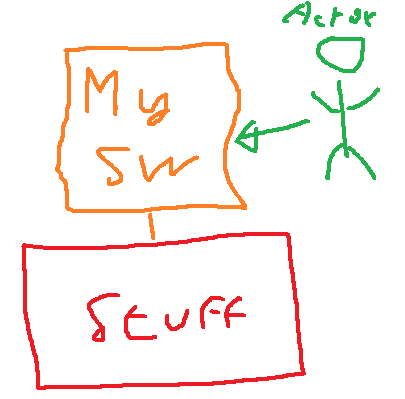
\includegraphics{architecture.png}
    \caption{Architecture diagram for SW.COMP1}
    \centering\label{fig:architecture-diagram}
    \end{figure}

    \blindtext[1]


    \level{0}{Specific requirements}

    \level{1}{Functionnal requirements}

    \blindtext[10]

    \level{2}{Input commands}

    \blindtext[1]

    \input{snip/SRD-REQ-00001}

    Note: see \ref{software-item-description} for details about this command.

    \level{2}{Performance requirements}
    \blindtext[1]

    \level{2}{Interface requirements}
    \blindtext[1]

    \input{snip/SRD-REQ-80000}
    Du texte en dessous pour préciser
    Une table...

    \level{2}{Operationnal requirements}
    \level{3}{Versionning}
    \input{snip/SRD-REQ-01000}

    \level{0}{Verification and validation}
    \level{1}{Requirements}
    \blindtext[10]

    \level{1}{Methods}
    \blindtext[10]

    \level{0}{Tracability matrices}\label{tracability-matrices}

    Test test
%    \input{snip/matrix_to_SP-PIDS}
%    \input{snip/SRD-REQ-00001.tex_table}

\end{document}
